\documentclass[draft,jgrga]{agutex}

%  Uncomment the following command to include .eps files
\usepackage{graphicx}
%
%  Uncomment the following command to allow illustrations to print
%   when using Draft:
\setkeys{Gin}{draft=false}

% Author names in capital letters:
\authorrunninghead{HINES AND HETLAND}

% Shorter version of title entered in capital letters:
\titlerunninghead{RHEOLOGIC CONSTRAINTS ON THE MANTLE}

%Corresponding author mailing address and e-mail address:
\authoraddr{Corresponding author: T. T. Hines,
Department of Earth and Environmental Sciences, University of
Michigan, 2534 C. C. Little Building, 1100 North University Avenue,
Ann Arbor, MI 48109-1005. (hinest@umich.edu)} 

\begin{document}

\title{Supporting Information for ``Rheologic constraints on the upper mantle from five years of postseismic deformation following the El Mayor-Cucapah earthquake"}

\authors{Trever T. Hines,\altaffilmark{1}
         Eric A. Hetland,\altaffilmark{1}}

\altaffiltext{1}{Department of Earth and Environmental Sciences, University of Michigan, Ann Arbor, Michigan, USA.}

\begin{article}

\noindent\textbf{Contents of this file}
%%%Remove or add items as needed%%%
\begin{enumerate}
\item Figures S1 to S4
\end{enumerate}
\noindent\textbf{Introduction}

Figures S1 and S2 provide additional information about the inversion in Section 3.2 of the main text. Figures S3 and S4 show the predicted displacements, which have been decomposed into elastic and viscoelastic components, for the preferred model from Section 3.3.  
  
\end{article}
\clearpage

% Delete all unused file types below. Copy/paste for multiples of each file type as needed.

% enter figures and tables here:
\begin{figure}
\setfigurenum{S1} %%Change number for each figure
\noindent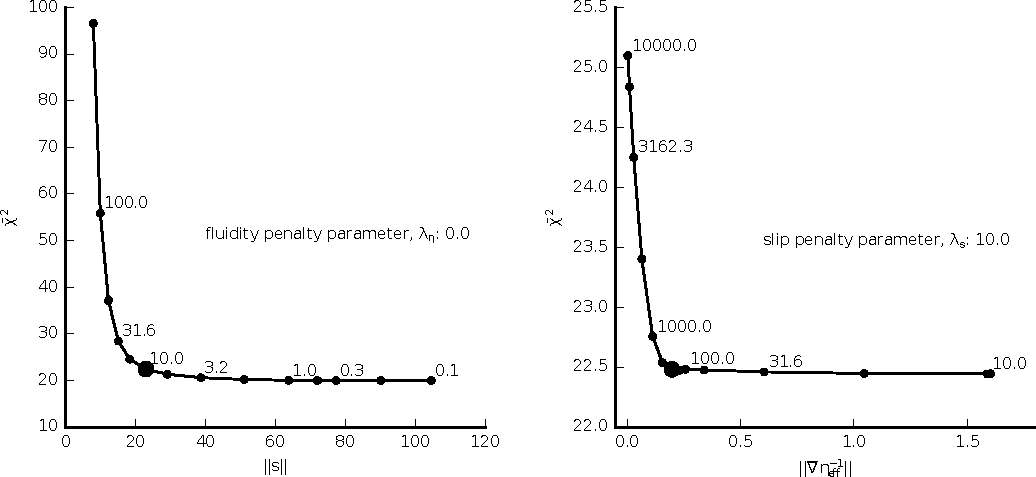
\includegraphics[scale=1.0]{Figures/2016jb013114-fS01}
\caption{
Trade-off curves used to determine the damping parameters $\lambda_s$ and $\lambda_\eta$ in eq. (15) of the main text.  The left panel shows the trade-off curve for the fault slip penalty parameter, $\lambda_s$.  We pick $\lambda_s$ while keeping the penalty parameter for fluidity, $\lambda_\eta$, fixed at zero.  The right panel shows the trade of curve for selecting $\lambda_\eta$, where we fix $\lambda_s$ at the chosen value from the left panel. Chosen values are indicated with the larger marker.  When picking $\lambda_s$, we try to find a good balance between the mean chi-squared value, $\bar{\chi}^2$, and the size of the slip parameters, $||s||$.  Our choice of $\lambda_\eta$ is a balance between $\bar{\chi}^2$ and the size of the Laplacian of fluidity, $||\nabla \eta_\mathrm{eff}^{-1}||$. 
}
\label{fig:S1}
\end{figure}

\begin{figure}
\setfigurenum{S2} %%Change number for each figure
\noindent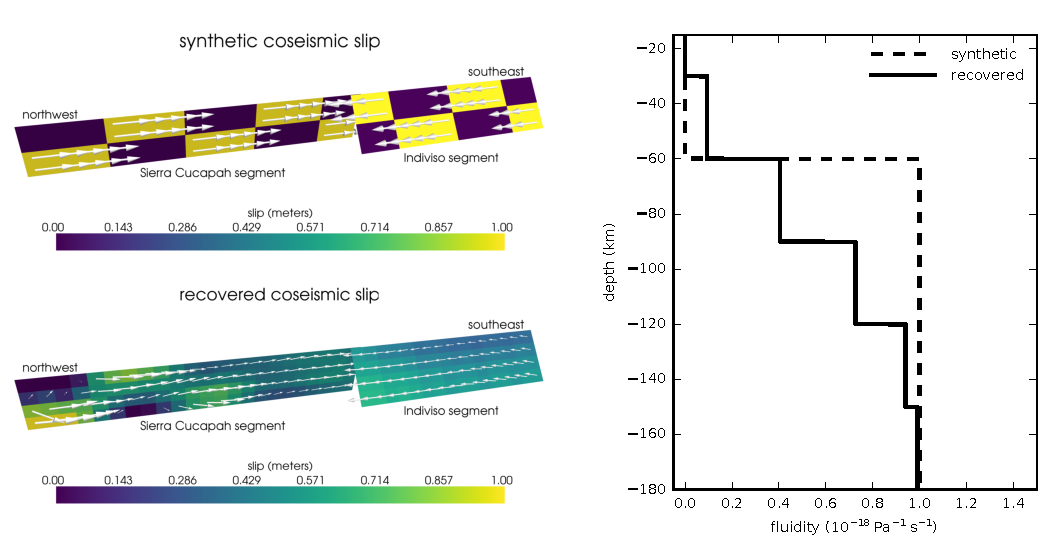
\includegraphics[scale=1.0]{Figures/2016jb013114-pS02}
\caption{
Checkerboard test used to assess the resolving power of the inversion in Section 3.2 of the main text.  We create synthetic data at all of the GPS stations considered in this study by evaluating eq. (14) with the synthetic coseismic slip distribution and fluidity distributions. Our synthetic fluidity model has a jump from 0.0 to $10^{-18}$ Pa$^{-1}$ s$^{-1}$ at 60 km depth.  Our synthetic slip model does not include afterslip, although we estimate afterslip along with coseismic slip and fluidity in this test.  We estimate these values in the same way as described in the main text and we also use the same penalty parameters.  We do not add any noise to our synthetic data so that the recovered model just indicates how much the regularization influences the solution.  Note that our ability to recover slip decreases towards the southern end of the fault, farthest from the available data.  Also note that the smoothing constraint on fluidity largely obscures the jump in the synthetic model.
}
\label{fig:S2}
\end{figure}

\begin{figure}
\setfigurenum{S3} %%Change number for each figure
\noindent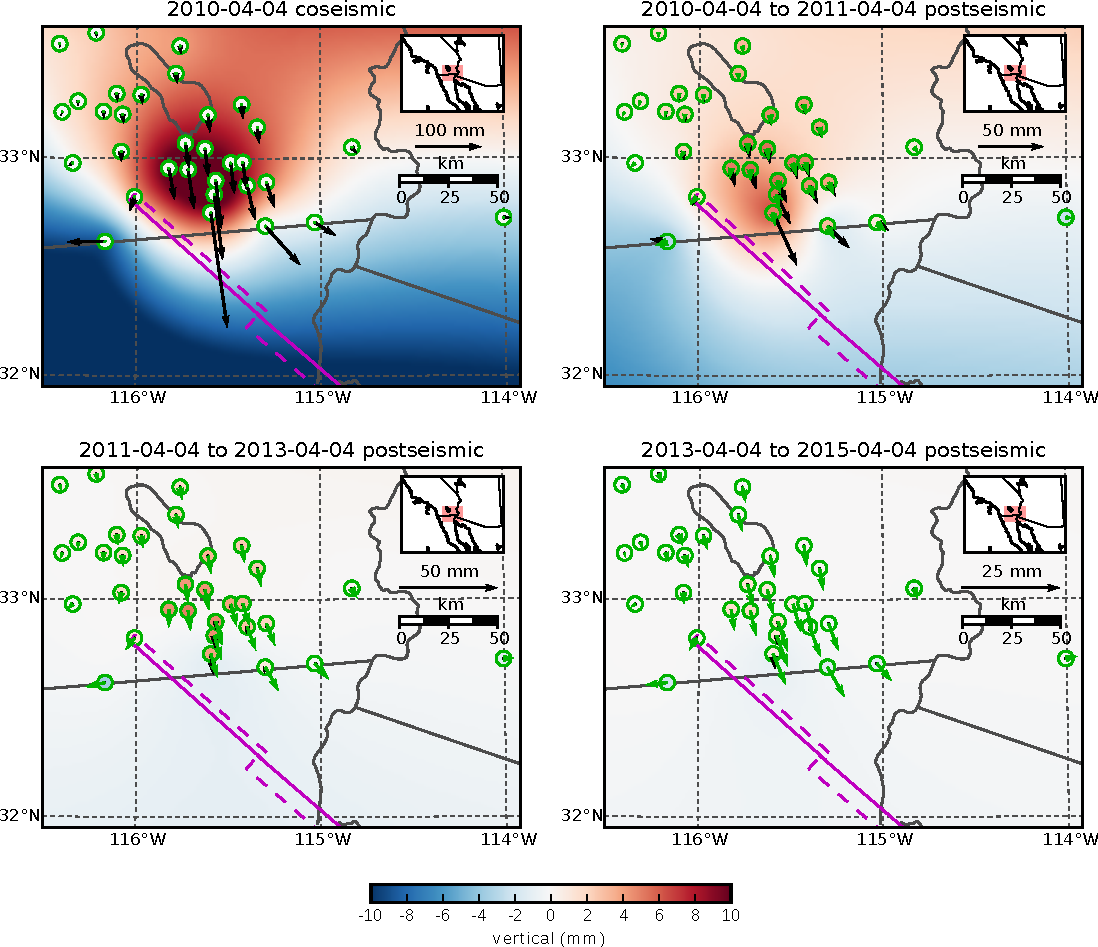
\includegraphics[scale=0.9]{Figures/2016jb013114-pS03}
\caption{
Elastic (black) and viscoelastic (green) components of the near-field predicted displacements for the preferred Zener model from Section 3.3.  The vertical elastic component is shown as an interpolated field and the vertical viscoelastic components are shown within the green circles.  The elastic and viscoelastic components are calculated from the first and second term in eq. (11).  The elastic component can be interpreted as the displacements resulting from fault slip and the viscoelastic component can be interpreted as the displacement due to relaxation of stresses induces by the slip. 
}
\label{fig:S3}
\end{figure}

\begin{figure}
\setfigurenum{S4} %%Change number for each figure
\noindent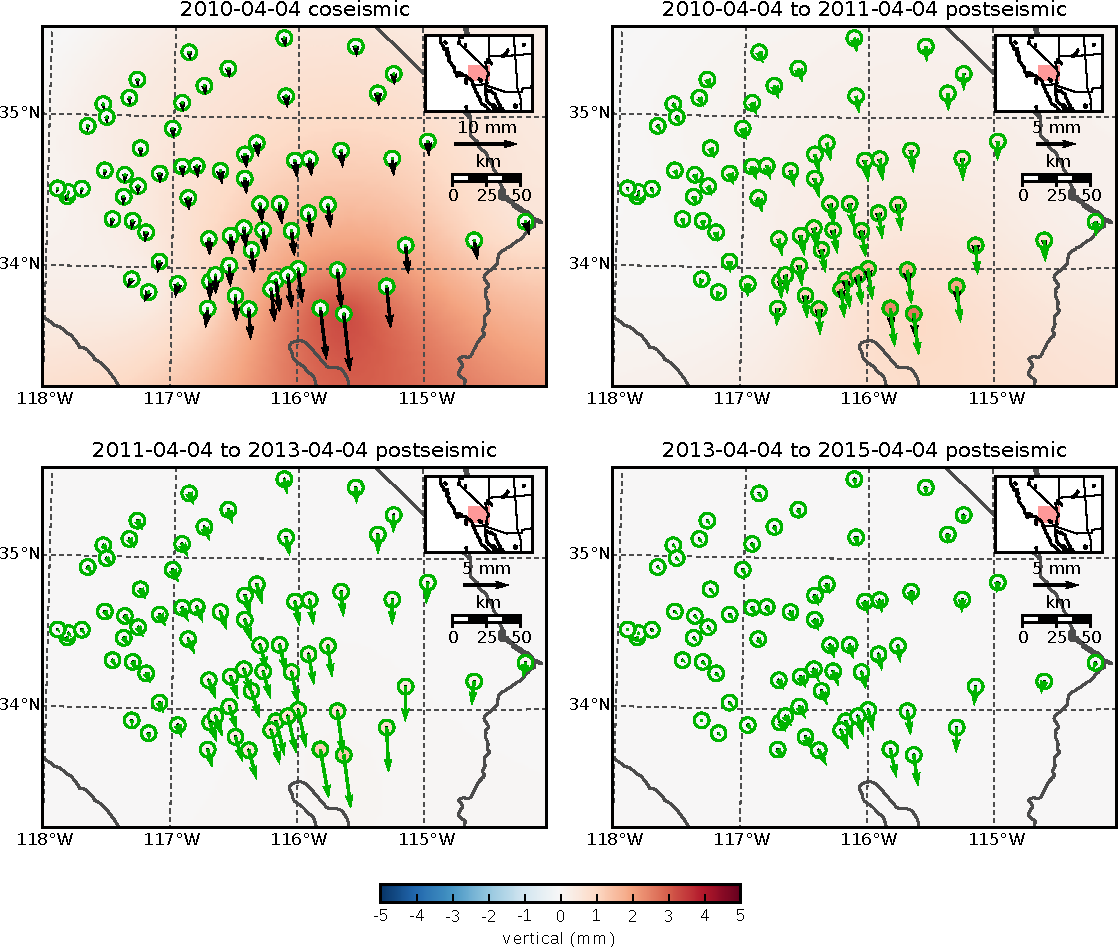
\includegraphics[scale=0.9]{Figures/2016jb013114-pS04}
\caption{
Same as figure S3 but for far-field stations.
}
\label{fig:S4}
\end{figure}

\end{document}

%%%%%%%%%%%%%%%%%%%%%%%%%%%%%%%%%%%%%%%%%%%%%%%%%%%%%%%%%%%%%%%

More Information and Advice:

%% ------------------------------------------------------------------------ %%
%
%  SECTION HEADS
%
%% ------------------------------------------------------------------------ %%

% Capitalize the first letter of each word (except for
% prepositions, conjunctions, and articles that are
% three or fewer letters).

% AGU follows standard outline style; therefore, there cannot be a section 1 without
% a section 2, or a section 2.3.1 without a section 2.3.2.
% Please make sure your section numbers are balanced.
% ---------------
% Level 1 head
%
% Use the \section{} command to identify level 1 heads;
% type the appropriate head wording between the curly
% brackets, as shown below.
%
%An example:
%\section{Level 1 Head: Introduction}
%
% ---------------
% Level 2 head
%
% Use the \subsection{} command to identify level 2 heads.
%An example:
%\subsection{Level 2 Head}
%
% ---------------
% Level 3 head
%
% Use the \subsubsection{} command to identify level 3 heads
%An example:
%\subsubsection{Level 3 Head}
%
%---------------
% Level 4 head
%
% Use the \subsubsubsection{} command to identify level 3 heads
% An example:
%\subsubsubsection{Level 4 Head} An example.
%
%% ------------------------------------------------------------------------ %%
%
%  IN-TEXT LISTS
%
%% ------------------------------------------------------------------------ %%
%
% Do not use bulleted lists; enumerated lists are okay.
% \begin{enumerate}
% \item
% \item
% \item
% \end{enumerate}
%
%% ------------------------------------------------------------------------ %%
%
%  EQUATIONS
%
%% ------------------------------------------------------------------------ %%

% Single-line equations are centered.
% Equation arrays will appear left-aligned.

Math coded inside display math mode \[ ...\]
 will not be numbered, e.g.,:
 \[ x^2=y^2 + z^2\]

 Math coded inside \begin{equation} and \end{equation} will
 be automatically numbered, e.g.,:
 \begin{equation}
 x^2=y^2 + z^2
 \end{equation}

% IF YOU HAVE MULTI-LINE EQUATIONS, PLEASE
% BREAK THE EQUATIONS INTO TWO OR MORE LINES
% OF SINGLE COLUMN WIDTH (20 pc, 8.3 cm)
% using double backslashes (\\).

% To create multiline equations, use the
% \begin{eqnarray} and \end{eqnarray} environment
% as demonstrated below.
\begin{eqnarray}
  x_{1} & = & (x - x_{0}) \cos \Theta \nonumber \\
        && + (y - y_{0}) \sin \Theta  \nonumber \\
  y_{1} & = & -(x - x_{0}) \sin \Theta \nonumber \\
        && + (y - y_{0}) \cos \Theta.
\end{eqnarray}

%If you don't want an equation number, use the star form:
%\begin{eqnarray*}...\end{eqnarray*}

% Break each line at a sign of operation
% (+, -, etc.) if possible, with the sign of operation
% on the new line.

% Indent second and subsequent lines to align with
% the first character following the equal sign on the
% first line.

% Use an \hspace{} command to insert horizontal space
% into your equation if necessary. Place an appropriate
% unit of measure between the curly braces, e.g.
% \hspace{1in}; you may have to experiment to achieve
% the correct amount of space.


%% ------------------------------------------------------------------------ %%
%
%  EQUATION NUMBERING: COUNTER
%
%% ------------------------------------------------------------------------ %%

% You may change equation numbering by resetting
% the equation counter or by explicitly numbering
% an equation.

% To explicitly number an equation, type \eqnum{}
% (with the desired number between the brackets)
% after the \begin{equation} or \begin{eqnarray}
% command.  The \eqnum{} command will affect only
% the equation it appears with; LaTeX will number
% any equations appearing later in the manuscript
% according to the equation counter.
%

% If you have a multiline equation that needs only
% one equation number, use a \nonumber command in
% front of the double backslashes (\\) as shown in
% the multiline equation above.

%% ------------------------------------------------------------------------ %%
%
%  SIDEWAYS FIGURE AND TABLE EXAMPLES
%
%% ------------------------------------------------------------------------ %%
%
% For tables and figures, add \usepackage{rotating} to the paper and add the rotating.sty file to the folder.
% AGU prefers the use of {sidewaystable} over {landscapetable} as it causes fewer problems.
%
% \begin{sidewaysfigure}
% \includegraphics[width=20pc]{samplefigure.eps}
% \caption{caption here}
% \label{label_here}
% \end{sidewaysfigure}
%
%
%
% \begin{sidewaystable}
% \caption{}
% \begin{tabular}
% Table layout here.
% \end{tabular}
% \end{sidewaystable}
%
%

